\documentclass[11pt,a4paper]{article}
\usepackage[utf8x]{inputenc}
\usepackage[T1]{fontenc}
%\usepackage{gentium}
\usepackage{mathptmx} % Use Times Font

\usepackage{graphicx} % Required for including pictures
\usepackage{hyperref} % Format links for pdf
\usepackage[british]{babel} % Multilingual bibliographies
\usepackage{natbib}
\setlength{\bibsep}{0.0pt}

\frenchspacing % No double spacing between sentences
\usepackage[margin=1in]{geometry}

\usepackage[all]{nowidow} % Tries to remove widows
\usepackage[protrusion=true,expansion=true]{microtype} % Improves typography, load after fontpackage is selected

\usepackage{lipsum} % Used for inserting dummy 'Lorem ipsum' text into the template

\title{Popularity of Munros}
\author{Filip Balucha, Advaith Sai Maddipatla, Tudor Finaru}
%\usepackage{natbib}

\begin{document}

\maketitle

%% INSTRUCTIONS:
%%
%% 1. Please rename this file fds-project-option-1.tex,
%% fds-project-option-2.tex, or fds-project-option-3.tex, depending on
%% which project option you are doing. When you submit, please submit
%% the PDF file with the corresponding name.
%% 
%% 2. You can edit either using:
%%
%%    a. Overleaf professional, a collabaratorive LaTeX editor. See
%%       https://www.overleaf.com/edu/edinburgh for documentation. Create an
%%       empty document, and copy the files in this directory to it.
%%
%%    b. A LaTeX editor on your PC - you can commit changes to this
%%       repository to collaborate.
%% 
%% 3. Please keep the section and paragraph headings as they are.
%%
%% 4. The word limit for the Overview section is mandatory. For the
%% other sections word limits are suggested.
%%
%% 5. The page limits must be strictkly adhered to, and depend on if
%% you are working individually, in pairs or in threes:
%%
%%   - Individual: 6 pages 
%%   - Pairs: 8 pages 
%%   - Threes: 10 pages 
%%

\section{Overview}
% 250 words maximum
Description of problem, work carried out, and results

\section{Introduction}
% Suggested 400 words

\paragraph{Context and motivation}

What is the area of this data science study, and why is it interesting
to investigate?

\medskip 

This study aims to shed light on 

\paragraph{Previous work}

Brief description of any previous work in this area (e.g., in the
media, or scientific literature or blogs).

E.g. Recent surveys show that most students prefer final projects to
final exams \cite{Space2021}. 

\paragraph{Objectives}

What questions are you setting out to answer?

\medskip
We are setting out to answer the following questions:

\begin{itemize}
    \item Is there a statistically significant relationship between Munro height and frequency of climb?
\end{itemize}

\section{Data}
% Suggested 300 words

\paragraph{Data provenance} Who created the dataset(s)?  How you have
obtained it (e.g., file or web scraping), and do the T\&Cs allow you
to use obtain the data for the project?

\medskip
We used three datasets: 
\begin{itemize}
    \item WalkHighlands (WH), from which we extracted data on the popularity, rating and accessibility of Munros. This data relies on contributions from registered users - they can select Munros they have climbed and rate them. We retrieved the data using web scraping for the main Munro tables and subpages; additionally, we manually copied the accommodation counts from the relevant subpages. These methods were chosen after a careful assessment of the T\&Cs.
    \item The Database of British and Irish Hills (DoBIH), from which we extracted geographical data on the Munros. The origins of this data can be traced in a 'series of articles in Marhofn and Relative Matters magazine', according to the website. The current editorial team consists of Graham Jackson, Chris Crocker, John Barnard, Simon Edwardes, George Gradwell, Jim Bloomer, and Dave Marshall. The T\&Cs of this dataset are quite liberal, as they impose 'no restrictions on use of the data by third parties', so long as the terms of the Creative Commons license are respected. Retrieving the data was easy, as it only involved downloading a readily available CSV file.
    \item Simplemaps Cities Database (SCD), from which we extracted data on British cities' location and population. The data comes from the US National Geospatial-Intelligence Agency, and is freely available to use under an MIT license. Again, retrieving the data only involved downloading a CSV file.
\end{itemize}

\bigskip 

All web scraping was performed in accordance with James Densmore's rules for ethical web scraping \cite{EiWS}:
\begin{itemize}
    \item We only scraped data when necessary - i.e. if no file or API was accessible.
    \item We always provided a “User Agent” string to make our intentions clear to the site owner, as well as to provide a way to contact the team member responsible for data processing.
    \item We requested data at a reasonable rate of at most 1 request per 10 seconds.
    \item We only saved the data we absolutely needed.
    \item We respected all data we obtained, and we did not pass it off as our own.
\end{itemize}

\paragraph{Data description} Description of the data, e.g. variables
in each table, number of records.
    
\medskip
After processing the data and joining the resulting tables (the details of these operations are presented in the 'Data processing' section), we reached the following variables (as seen in Table~\ref{table:1}):


\begin{table}
    \centering
     \begin{tabular}{||c | c | c||} 
     \hline
     Variable & Type & Description  \\ 
     \hline\hline
     name & string & the name of the Munro \\ 
     \hline
     altitude & integer & the altitude of the Munro in metres \\
     \hline
     ascent\_count & integer & the number of times the Munro was ascended by WH \\
     \hline
     rating & float[0,5] & munro rating from WH users normalised using Bayesian average \\
     \hline
     region & string & the region in which the Munro is located \\
     \hline 
     rating\_count & integer & the number of ratings for the Munro \\
     \hline 
     report\_count & integer & number of reports (i.e. mini blog posts) from WH users for the Munro \\
     \hline 
     hotel\_count & integer & number of hotels in the region \\
     \hline 
     bb\_count & integer & number of B\&Bs in the region \\
     \hline 
     cottage\_count & integer & number of cottages in the region \\
     \hline
     hostel\_count & integer & number of hostels in the region \\
     \hline
     camping\_count & integer & number of camping and glamping sites in the region \\
     \hline
     neighbor\_count\_<radius> & integer & number of neighboring Munros within a given radius \\
     \hline 
     nearest\_city\_dist & float (2 d.p.) & haversine distance to the city closest to the Munro \\
     \hline
     nearest\_city\_population & integer & population of the city closest to the Munro \\
     \hline 
     nearest\_large\_city\_dist & float (2 d.p.) & haversine distance to a large city (i.e. above 50K) closest to the Munro \\
     \hline 
     population\_<radius> & integer & the sum of populations of all cities within a given radius \\
     \hline
    \end{tabular}
    \caption{Variables}
    \label{table:1}
\end{table}

\paragraph{Data processing} How you have processed the dataset, e.g.,
cleaning, removing missing values, joining tables.

\medskip 

After scraping the WH data, we normalised the ratings since the rating count presented wild variations (taking values between 22 and 317). We computed the Bayesian average, which pulls ratings that are based on few votes closer to the mean rating. It uses two fields: m, the prior mean, i.e. the mean rating for all Munros, and C, the number of ratings required for a decent estimate of the sample mean. In other words, C is the number of observations necessary to “get away” from m. These values were eyeballed from a joint distribution plot of “rating” and “rating\_count” to be m := 3.6 and C := 60.

\smallskip
For the DoBIH data, we first filtered out irrelevant columns, then chose only Munros using the boolean tag 'M'. Additionally, we changed the column naming to snake\_case for consistency.

\smallskip
For the SCD data, we first filtered out cities not in the UK and cities with a population of less than 100. Then, for each Munro, we computed the distance to and population of the nearest city, as well as the distance to the nearest large city and the total population within a certain radius from the Munro. We treated the islands of Mull and Skye separately, since neither Portree nor Tobermory, their corresponding largest settlements, are in the database. Considering that Skye is connected to the mainland via a road bridge, we considered the impact of mainland cities on the popularity of Skye Munros. However, since Mull is isolated from the mainland, we simply replaced all city-related values with NaN.

\medskip 
Merging the WH and DoBIH datasets was a challenging - yet very rewarding - process. First of all, we created a unique key for each Munro in both tables. The key of choice was a stringified tuple consisting of name and altitude, since only these two fields are available in both datasets. Sadly, they did not always match exactly - some particular cases were so bad that they needed to be handled manually (e.g. the name “Carn Dearg” appears in DoBIH three times). For the remaining data, we performed fuzzy matching on the keys i.e. we matched a key from WH to the closest key in DoBIH based on edit-distance.  We used `difflib` for this purpose. We then merged the data and removed unnecessary fields such as the aforementioned keys.

After merging, we computed the number of neighbours for each Munro; that is, the number of Munros located within a radius of 1, 2.5, 5, 10, 15, and 20 km (using the haversine distance). We only considered Munros located on the same land mass, since we assume that a climber who is to climb multiple Munros in a restricted area will not want to drive to another island to do so (e.g. Skye).

\section{Exploration and  analysis}
% Suggested 500 words for individual report; proportionately longer
% for group projects).

To address the first question, we start by visualising the distributions of Munro ascent counts and heights. Figure \ref{fds-project-template:fig:ascent_dis} and Figure \ref{fds-project-template:fig:altitude_dis} show the individual distributions of Munros in relation to the two variables:

\begin{figure}[h!]
   \begin{minipage}{0.48\textwidth}
     \centering
     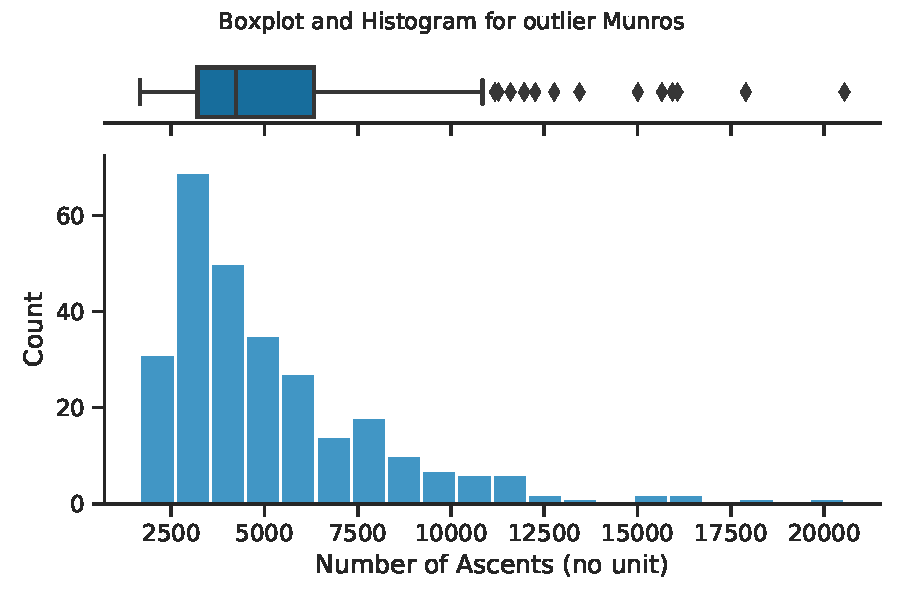
\includegraphics[width=1.2\linewidth]{report/ascent_distribution.pdf}
     \caption{Distribution of Munros by ascent count.}
     \label{fds-project-template:fig:ascent_dis}
   \end{minipage}\hfill
   \begin{minipage}{0.48\textwidth}
     \centering
     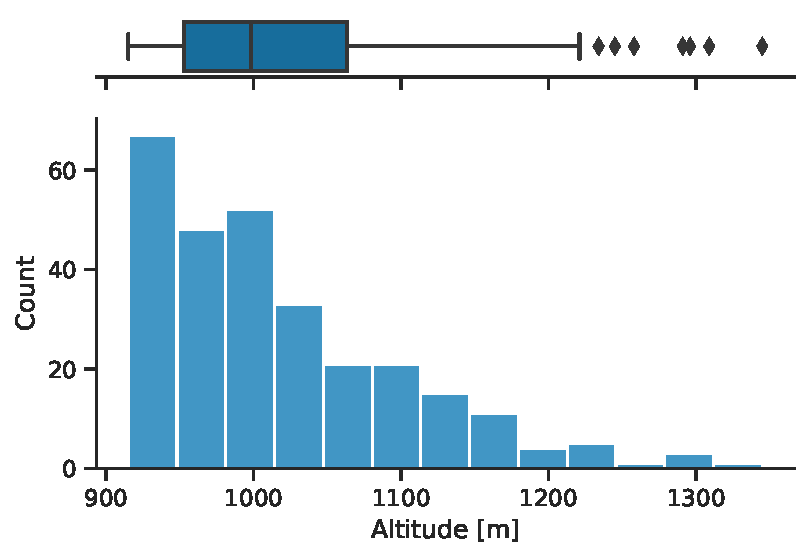
\includegraphics[width=1.2\linewidth]{report/altitude_distribution.pdf}
     \caption{Distribution of Munro heights.}
     \label{fds-project-template:fig:altitude_dis}
   \end{minipage}
\end{figure}


We wish to get a summary view of both variables at once. To that end, we plot the joint distribution of altitude and ascent count as seen in Figure \ref{fds-project-template:fig:heatmap}.

\begin{figure} [h!]
  \centering
  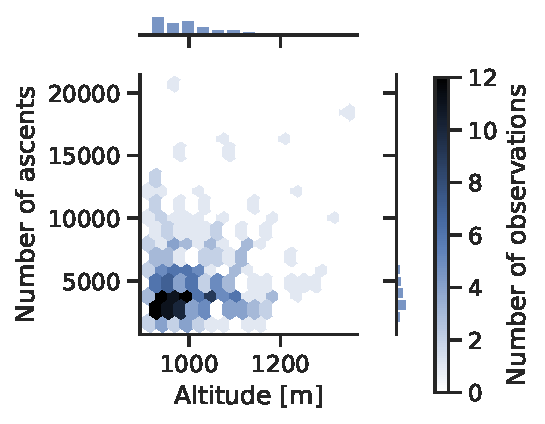
\includegraphics{report/heatmap_joint_distribution.pdf}
  \caption{Joint distribution of Munro heights and ascent counts.}
  \label{fds-project-template:fig:heatmap}
\end{figure}

\medskip 

\begin{figure} [h!]
  \centering
  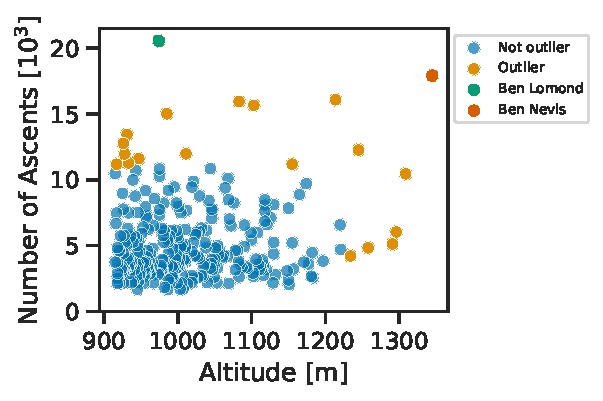
\includegraphics{report/scatterplot.pdf}
  \caption{Scatterplot of ascent count and altitude with key outliers highlighted.}
  \label{fds-project-template:fig:scatterplot}
\end{figure}

Figure \ref{fds-project-template:fig:heatmap} shows that most Munros have an altitude situated between 900 and 1000m, and an ascent count of 2500 to 3000. There exist a number of apparent outliers in the data - as was also visible in the boxplots attached to Figure \ref{fds-project-template:fig:altitude_dis} and Figure \ref{fds-project-template:fig:ascent_dis}. In order to better understand and identify some key outliers, it is worth having a look at a scatterplot of ascent count and altitude, as seen in Figure \ref{fds-project-template:fig:scatterplot}.

\medskip

It comes as little surprise that the two most popular Munros are Ben Lomond and Ben Nevis. In fact, the former takes the top spot despite having a height of less than 1000 metres. This could likely be explained by its extraordinary popularity with the people of Glasgow, Scotland's most populous city. Ben Lomond is within easy reach of said city, and is well-known as an accessible spot of natural beauty for Glaswegians. Ben Nevis' significant popularity was expected given its status as the tallest mountain in Britain. Its relatively isolated location in the North-West of Scotland does little to deter plenty of people from all over the UK from attempting the comparatively strenuous hike.

\medskip 

We are now in a better position to answer our initial question. Judging by Figure \ref{fds-project-template:fig:scatterplot}, there appears to be no clear relationship between Munro altitude and ascent count. However, the outliers (e.g. Ben Nevis) should exert a leverage and thus we can still expect to see a positive relationship between number of ascents and altitude. Nevertheless, our conclusions will unfortunately be marred by the large variance in the left-hand side of the scatterplot.

\bigskip

We use hypothesis testing. The null and alternate hypotheses are as follows:

H\textsubscript{0} = There is not a statistically significant relationship between altitude and number of ascents.

H\textsubscript{1} = There is a statistically significant relationship between altitude and number of ascents.

\bigskip

We apply linear regression using the Least Squares method and observe the results of statsmodels, which produces the following error message: 'The condition number is large, 1.25e+04. This might indicate that there are
strong multicollinearity or other numerical problems'. Since we are only using a single predictor, multicollinearity is out of the questions - which means we need to deal with the numerical instability. We remedy the instability by centering the independent variable around 0.


\medskip 

Applying linear regression on the processed data yields the prediction seen in Figure \ref{fds-project-template:fig:q1_prediction}. 

\begin{figure} [h!]
  \centering
  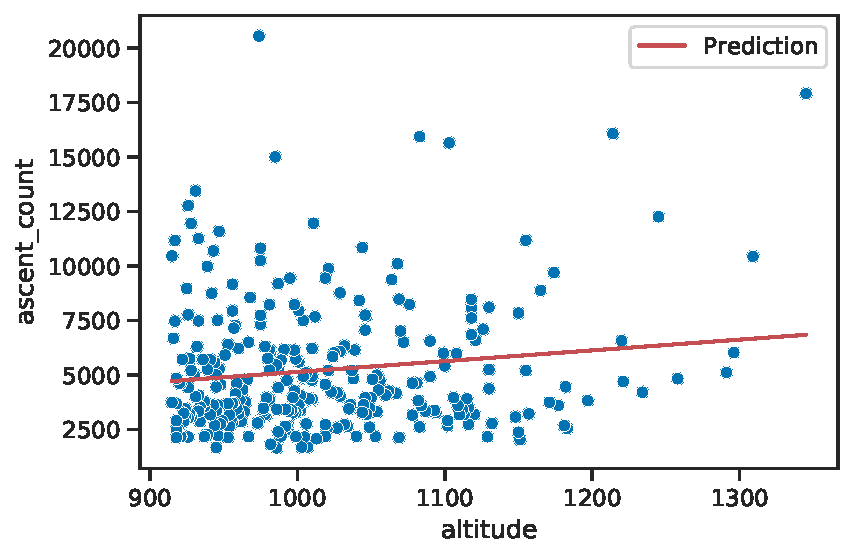
\includegraphics{report/q1_prediction.pdf}
  \caption{Prediction over centered data}
  \label{fds-project-template:fig:q1_prediction}
\end{figure}

\medskip

Again, we note some important results from statsmodels. The p-value tells us that there is a 2\% probability that the relationship between altitude and ascent count may be due to chance. Since 0.021 < 0.05, it allows us to reject the null hypothesis that the coefficient of altitude in the model equals 0 at the 5\% level. Furthermore, the t score is fairly high too, which further asserts our claim. Thus, there is a statistically significant relationship between altitude and ascent count. However,we observe that the R\textsuperscript{2} value is quite low at 0.019. This tells us that the model does not fit the data too well. This motivates the use of further predictors to aid our analysis.

\medskip 

Since we standardised the independent variable (i.e. it has mean 0), the intercept tells us the expected ascent count for a Munro of mean altitude - which is 5233.8. We now compute the root mean squared error to assess how far off our predictions are from the target values in absolute terms on average. The RMSE indicates how far our predictions of ascent count deviate from actual observed values, in absolute terms - and in our case, they deviate by about 3000. Given that the mean ascent count is approximately 5200, this is a a relatively large number.

\medskip

This can perhaps be explained by looking at the residuals distribution as seen in Figure \ref{fds-project-template:fig:residuals_dist}.

\begin{figure} [h!]
  \centering
  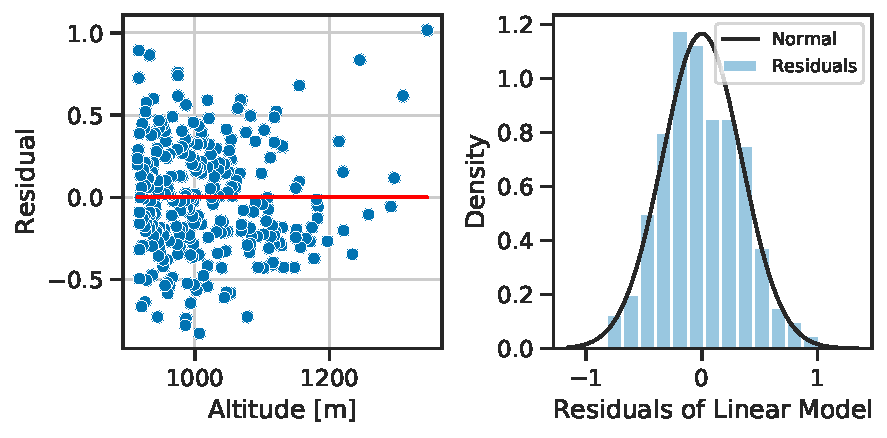
\includegraphics{report/residuals_dist.pdf}
  \caption{Distribution of Residuals}
  \label{fds-project-template:fig:residuals_dist}
\end{figure}

A good Linear regression fit requires the residuals to be normally distributed. This is not exactly a normal distribution, and is fairly skewed; this is not what we are looking for. We now plot residuals against altitude to check for a potential relationship - the results are seen in Figure \ref{fds-project-template:fig:residuals_plot}.

\begin{figure} [h!]
  \centering
  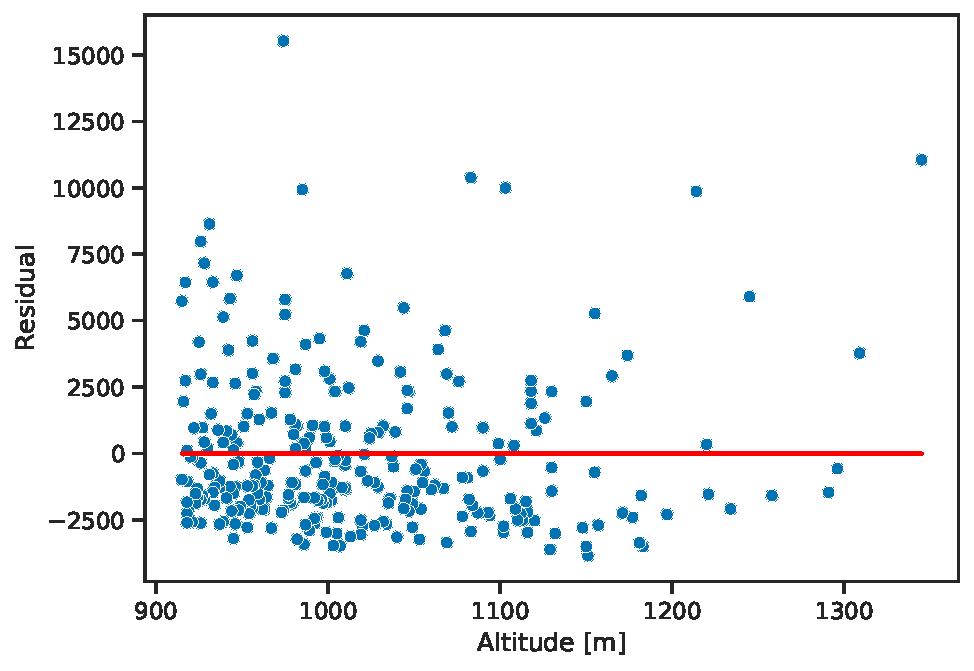
\includegraphics{report/residuals_plot.pdf}
  \caption{Residuals and Altitude Plot}
  \label{fds-project-template:fig:residuals_plot}
\end{figure}

% EXPERIMENT START
\begin{figure} [h!]
  \centering
  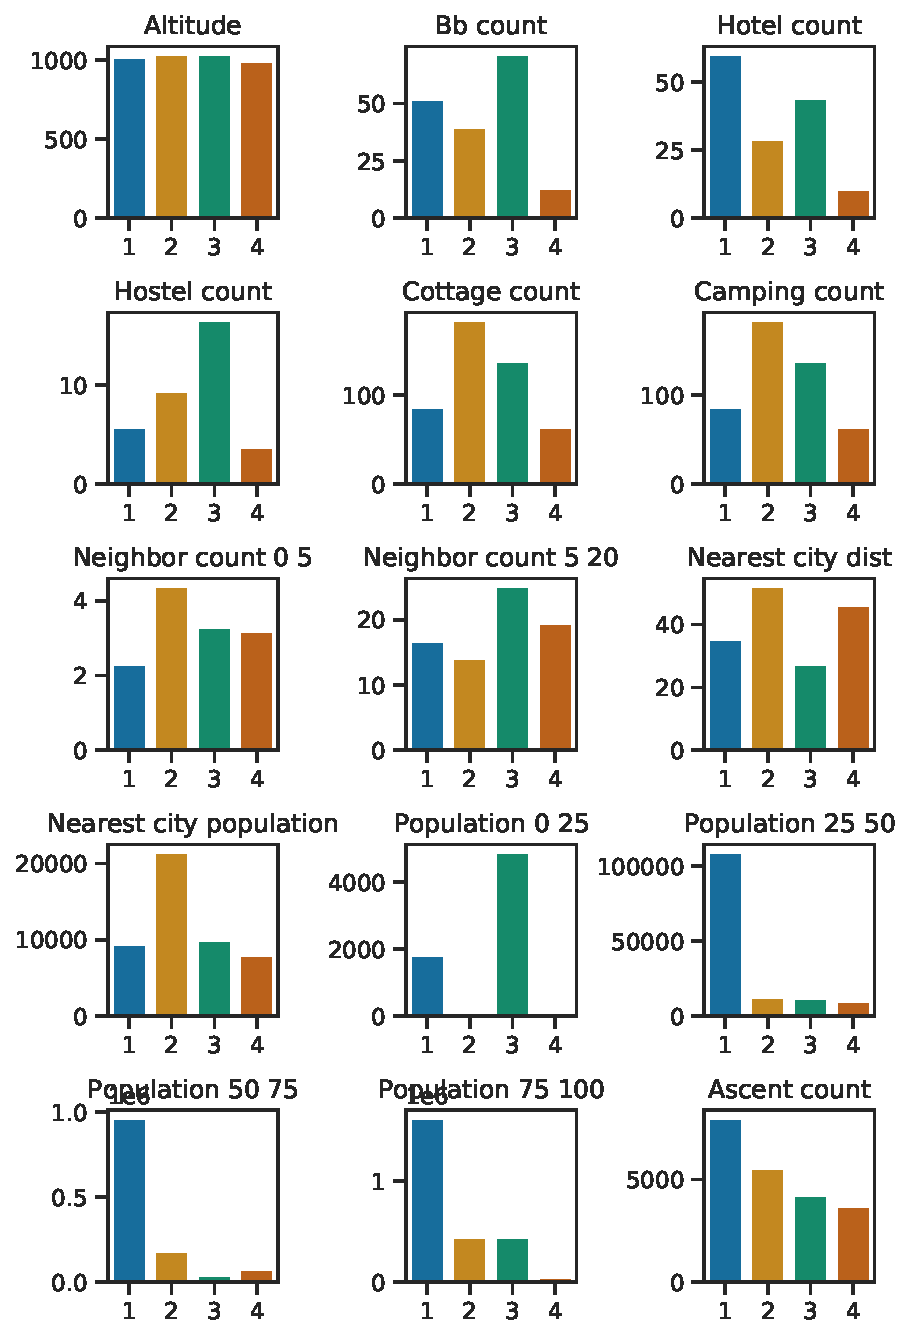
\includegraphics{report/munro_features.pdf}
  \caption{TBA}
  \label{fds-project-template:fig:scatterplot}
\end{figure}

\begin{figure} [h!]
  \centering
  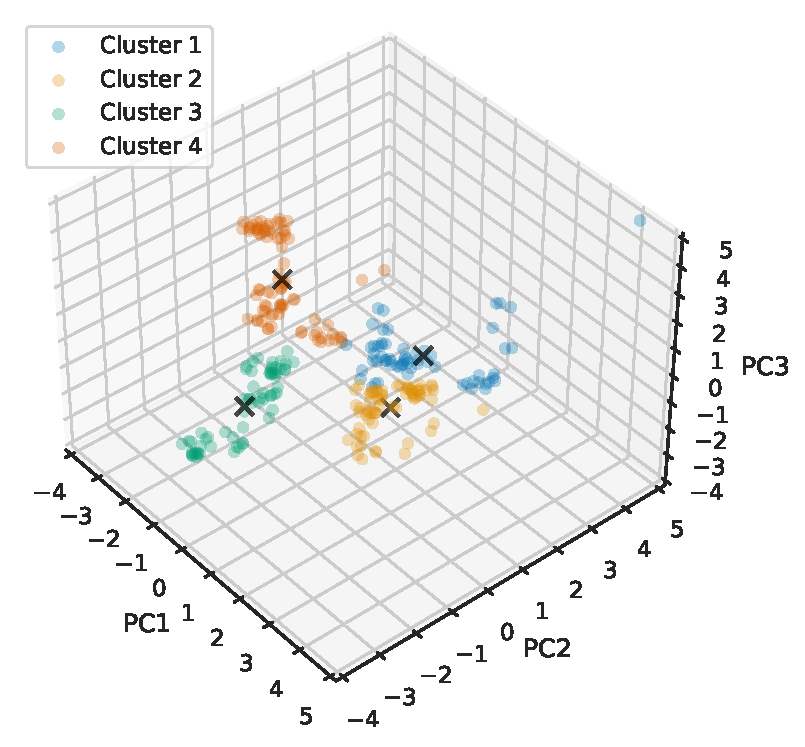
\includegraphics{report/3d_clusters.pdf}
  \caption{TBA}
  \label{fds-project-template:fig:scatterplot}
\end{figure}
% EXPERIMENT END

\medskip 

The plot is not heteroskedastic. Additionally, there is no discernible pattern – the independent variable and variance do not exhibit a relationship. This tells us that the linear model we used earlier was not a bad choice for the given task.

\medskip 

Our conclusions should mostly be trustworthy; however, the nature of the data might affect their accuracy somewhat. Perhaps the most important thing to note is that we are working with the number of ascents by separate individuals as opposed to the frequency of climbs. Additionally, the data on the number of ascents has only been gathered from a single source - and WalkHighlands requires users to register before allowing them to contribute. This means that the group of people who contributed to the data we are using might not be fully representative of all hikers. The contributors can be expected to be active internet users with a real passion for hiking - which is not necessarily the case for every Munro climber.

% 't' means "try to position at the top of the page"
%\begin{figure}[t]
%  \centering
%  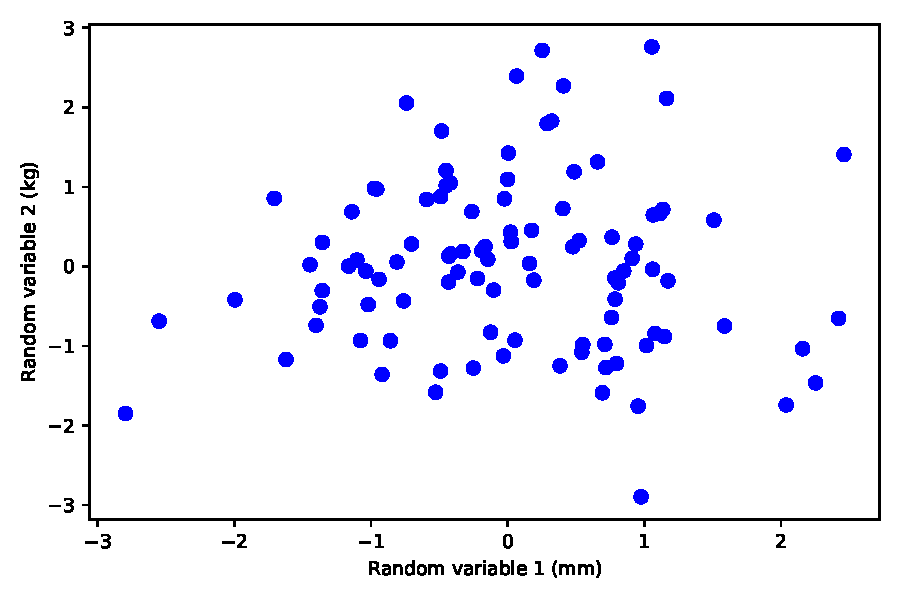
\includegraphics{example1}
%  \caption{Demonstration figure. This caption explains more about the
%    figure. Note that the font size of the labels in the plot is 9pt,
%    which is obtained by the settings as shown in the Jupyter
%    notebook.}
%  \label{fds-project-template:fig:example1}
%\end{figure}

% 'b' means "try to position at the bottom of the page"
\begin{table}[b]
  \caption{Exerpt from Scottish Index of Multiple Deprivation, 2016 edition.
    \url{https://simd.scot}. You may put more information in the caption.}
  \label{tab:example1}
\begin{tabular}{lrrrrrrr}
\hline\hline
\textbf{Location}&\textbf{Employ-}&\textbf{Illness}&\textbf{Attain-}&\textbf{Drive}  &\textbf{Drive}    &\textbf{Crime}&\dots\\
                 &\textbf{ment}   &                &\textbf{ment}   &\textbf{Primary}&\textbf{Secondary}&              &\\
\hline
\textbf{Macduff}&$10$&$ 95$&$5.3$&$1.5$&$6.6$&$249$&\dots\tabularnewline
\textbf{Kemnay}&$ 3$&$ 40$&$5.3$&$2.4$&$2.4$&$168$&\dots\tabularnewline
\textbf{Hilton}&$ 0$&$ 10$&$6.3$&$2.2$&$3.0$&$144$&\dots\tabularnewline
\textbf{Ruchill}&$ 8$&$130$&$4.9$&$1.7$&$5.6$&$318$&\dots\tabularnewline
\textbf{Belmont}&$ 2$&$ 50$&$6.1$&$3.1$&$3.2$&$129$&\dots\tabularnewline
\dots&\dots&\dots&\dots&\dots&\dots&\dots&\dots\tabularnewline
\hline
\end{tabular}
\end{table}

A data science analysis of the paper, including: 
\begin{itemize}
\item Visualisations (for example
  Figure~\ref{fds-project-template:fig:example1}) and tables (for
  example Table~\ref{tab:example1}). Please make sure that all figures
  and tables are referred to in the text, as demonstrated in this
  bullet point.
\item Interpretation of the results 
\item Description of how you have applied one ore more of the
  statistical and ML methods learned in the FDS to the data
\item Interpretation of the findings 
\end{itemize}

You can use equations like this:
\begin{equation}
  \label{fds-project-template:eq:1}
  \overline{x} = \sum_{i=1}^n x_i
\end{equation}
or maths inline: $E=mc^2$. However, you do not need to reexplain techniques that you have learned in the course -- assume the reader undertands linear regression, logicstic regression K-nerest neighbours etc.  Remember to explain any symbols use, e.g.~``$n$ is the number of data points and $x_i$ is the value of the $i$th data point.''.

\section{Discussion and conclusions}
% Suggested 400 words.

\paragraph{Summary of findings}

\paragraph{Evaluation of own work: strengths and limitations}

\paragraph{Comparison with any other related work}
E.g. ``Anscombe has also demonstrated that many patterns of data can
have the same correlation coefficient'' \cite{Ansc73Grap}.

\paragraph{Improvements and extensions}

\bibliographystyle{unsrt}
\bibliography{fds-project}
\end{document}
